%% thesis.tex 2014/04/11
%
% Based on sample files of unknown authorship.
%
% The Current Maintainer of this work is Paul Vojta.

\documentclass{ucbthesis}
%\usepackage{biblatex}
\usepackage[backend=biber, sorting=none]{biblatex}
\usepackage{rotating} % provides sidewaystable and sidewaysfigure
% all of the packages below are optional feel free to remove if you don't use them
\usepackage{textcomp} % degrees symbol
\usepackage{siunitx} % units
\usepackage{amsmath,amssymb,amsfonts,hyperref,lineno,microtype,setspace,multicol,textcomp, marvosym, algorithm,algpseudocode, algorithmicx, wrapfig}
\usepackage{booktabs, threeparttable, multirow} % Make pretty tables
\usepackage{caption} % for tables and figures
\captionsetup[table]{skip=4pt} % sets a default padding for tables
\usepackage{dsfont} % matrix notation
\usepackage{xr} % cross ref between files
\usepackage{lipsum} % for random text remove for your actual dissertation

% the code below is make a abs symbol and fraction without the bar
\usepackage{mathtools}
\DeclareRobustCommand\bfrac[2]{\genfrac{}{}{0pt}{}{#1}{#2}}
\DeclarePairedDelimiter\abs{\lvert}{\rvert}%
\DeclarePairedDelimiter\norm{\lVert}{\rVert}
% end of abs and custom frac

% this sets the color of hyperlinks
\hypersetup{colorlinks=true, citecolor=black, linkcolor=black, urlcolor=blue}

%footnote stuff -- this doesn't allow a footnote to spread across multiple pages
\interfootnotelinepenalty=10000
\renewcommand{\thefootnote}{\fnsymbol{footnote}}

% To compile this file, run "latex thesis", then "biber thesis"
% (or "bibtex thesis", if the output from latex asks for that instead),
% and then "latex thesis" (without the quotes in each case).

% Double spacing, if you want it.  Do not use for the final copy.
% \def\dsp{\def\baselinestretch{2.0}\large\normalsize}
% \dsp

% If the Grad. Division insists that the first paragraph of a section
% be indented (like the others), then include this line:
% \usepackage{indentfirst}

\addtolength{\abovecaptionskip}{\baselineskip}

\newtheorem{theorem}{Jibberish}

%\bibliography{thesis_1}
\addbibresource{thesis.bib} % if using biblatex

\hyphenation{mar-gin-al-ia}
\hyphenation{bra-va-do}

\begin{document}

% Declarations for Front Matter

\title{How to Ride Monsters}
\author{Brandon Wood}
\degreesemester{Summer}
\degreeyear{2019}
\degree{Doctor of Philosophy}
\chair{Professor Kelly Slater}
\othermembers{Professor Andy Irons\\
Professor John-John Florence}


% For a co-chair who is subordinate to the \chair listed above
% \cochair{Professor Benedict Francis Pope}
% For two co-chairs of equal standing (do not use \chair with this one)
% \cochairs{Professor Richard Francis Sony}{Professor Benedict Francis Pope}
\numberofmembers{3}
% Previous degrees are no longer to be listed on the title page.
% \prevdegrees{B.A. (University of Northern South Dakota at Hoople) 1978 \\
%   M.S. (Ed's School of Quantum Mechanics and Muffler Repair) 1989}
\field{Advanced Wave Riding}
% Designated Emphasis -- this is optional, and rare
% \emphasis{Colloidal Telemetry}
% This is optional, and rare
% \jointinstitution{University of Western Maryland}
% This is optional (default is Berkeley)
% \campus{Berkeley}

% For a masters thesis, replace the above \documentclass line with
% \documentclass[masters]{ucbthesis}
% This affects the title and approval pages, which by default calls this
% document a "dissertation", not a "thesis".

\maketitle
% Delete (or comment out) the \approvalpage line for the final version.
\approvalpage
\copyrightpage

% (This file is included by thesis.tex; you do not latex it by itself.)

\begin{abstract}

\setlength\parindent{20pt}
\setlength{\parskip}{0.08mm}
% The text of the abstract goes here.  If you need to use a \section
% command you will need to use \section*, \subsection*, etc. so that
% you don't get any numbering.  You probably won't be using any of
% these commands in the abstract anyway.

\noindent Never leave a good wave. Unless, there is a better one down the road. \lipsum[2]

\lipsum[2]


\end{abstract}


\begin{frontmatter}

\begin{dedication}
\null\vfil
\begin{center}
Dedication here\\\vspace{12pt}
\end{center}
\vfil\null
\end{dedication}

% You can delete the \clearpage lines if you don't want these to start on
% separate pages.

\tableofcontents
\clearpage
\listoffigures
\clearpage
\listoftables

\begin{acknowledgements}
Thank everyone here

\end{acknowledgements}

\end{frontmatter}

\pagestyle{headings}

% (Optional) \part{First Part}

\chapter{Introduction}

Throughout history there are numerous examples where materials discovery led to technological breakthroughs with significant societal impact: metals for early weaponry, filaments for incandescent light bulbs, catalysts for the Haber-Bosch process, and cathode materials for lithium-ion batteries to name only a few. Discovery of novel, functional materials remains one of the most important challenges for the fields of chemistry, material science, and condensed matter physics. The overarching goal of this thesis is to improve the design of organic materials and molecules using computational and theoretical methods.

In the late 1970’s, Shirakawa, MacDiarmid, and Heeger discovered that chemically doping (oxidizing) the conjugated polymer polyacetylene transforms it from an insulator to a metal-like material, increasing its electronic conductivity over 7 orders of magnitude \cite{Shirakawa1977}! This discovery inspired an entirely new field of scientific research based on organic electronics, promising many of the benefits of insulating polymers (e.g. fabrication potential) while possessing unique electronic properties. Indeed, as recognition of the impact, Shirakawa, MacDiarmid, and Heeger received the 2000 Noble Prize in Chemistry. In the years to follow, a wide range of related applications were explored, such as: organic light emitting diodes (OLEDs), organic transistors, organic solar cells, battery materials, biomedical devices, and flexible/wearable electronics \cite{Burroughes1990, Sarpeshkar2002, Gunes2007, Liang2012, SmelaE.2003, Oh2016}. Even more exotic functionalities have been theorized, such as neuromorphic computing and superconductors \cite{VanDeBurgt2018, Swager2017}. Despite these exciting discoveries and application areas, more research is necessary before conjugated materials can reach their full potential.

The electronic properties of conjugated molecules and polymers are governed by the structure of the conductive backbone. The term conjugation was coined in the 1890’s \cite{Thiele1899}, and it represents a bonding pattern of alternating single and double bonds. Polyacetylene is a model example of a conjugated system. The physical origin of this bonding pattern can be explained as a Peierls distortion \cite{Roth2013} from the ideal case where all bond lengths are equal. In order for these materials to be electronically conductive there needs to be electron delocalization, which can be understood by considering atomic orbitals. Conjugation involves the interaction of $p_z$-orbitals between a series of atoms (usually carbon) with $sp^2$-hybridized electronic orbitals. Neighboring atoms with $p_z$ orbitals form $\pi$-bonds and a series of atoms create a connected network of $\pi$-bonds. The side view in Fig.~\ref{fig:eddb} reveals the $\pi$-bonding pathways (colored blue) above and below the bithiophene atoms. While $\pi$-bonding allows for some delocalization, $\pi$-electrons remain semibound and current state-of-the-art conjugated materials still require doping or excitation to generate mobile carriers \cite{Nobel2000}.

\begin{figure*}[hbt!]
  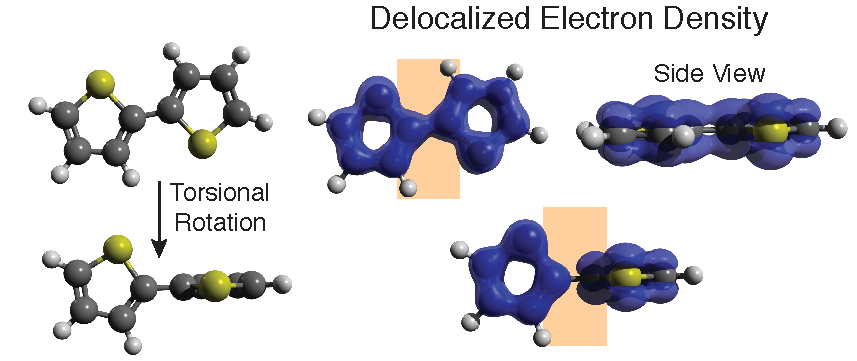
\includegraphics{figures/chap1_intro/figure_delocal_copy.pdf}
  \caption[Electron Density of Delocalized Bonds]{(Left) Two bithiophene torsional configurations, 180\textdegree \  (planar) on the top and 90\textdegree \ (non-planar) on the bottom. (Right) The electron density of delocalized bonds \cite{Szczepanik2017} isosurface plots (isovalue = 0.015). The isosurface of the non-planar configuration has a reduction in density between rings, which impacts its electronic properties. A side view of the planar configuration is included to display $\pi$-bonding pathways above and below the molecule.}
  \label{fig:eddb}
\end{figure*}

The atomic-scale structure of conjugated molecules and polymers plays a key role in determining carrier mobility and in turn electronic conductivity due to the geometric nature of $\pi$-bonding. In its completely planar undisturbed state, the $\pi$-bonding network in the electronic structure of the conjugated backbone provides an intramolecular conduction pathway for carriers. However, if a molecule or a chain is significantly torsioned (i.e. non-planar) the conduction pathway is disrupted. Figure \ref{fig:eddb} illustrates this point by comparing the delocalized electron density of a planar (top) and a non-planar (bottom) bithiophene torsional configuration. There is an electron deficient region between rings of the non-planar configuration, which represents a large energetic barrier that a carrier cannot overcome and hence represents a dead end for transport. These disruptions in conjugation are a product of polymer structure and limit carrier mobility and electronic conductivity.

As synthesized, conjugated polymer materials exhibit an intrinsic amount of structural disorder \cite{Noriega2013, Shen2016}, including non-planar configurations. This natural disorder introduces challenges for creating a micron-scale network of undisrupted pathways (i.e. no dead ends) for carrier transport. Although it is tempting to assume that more crystalline (i.e. ordered) materials would be more conductive, recent work indicates that less crystalline materials with undisrupted pathways are preferable \cite{Noriega2013, Son2016}. Part of the reason for this is that crystalline regions within the material are not guaranteed to align, creating many dead ends at the domain walls. Thus, a fundamental knowledge of structure, with predictive power at multiple length scales, is desirable to enable rationally designed engineering materials with undisrupted conjugation pathways. The central focus of this thesis is therefore to improve our understanding of amorphous (i.e. disordered) conjugated polymer structure at the electronic, atomic, and chain levels to inform design.

In Chapter 2 we concentrate on the topic of doped and excited polymer chain structure, utilizing a combination of quantum chemistry and statistical mechanics. Recent work by Son et al. and Noriega et al. demonstrate that carrier mobility in conjugated polymer materials is limited by the structure of the amorphous chains \cite{Noriega2013, Son2016}. Despite this fact, little is known about the impact doping or excitation have on the overall amorphous chain structure. To address this, we use a multiscale approach that captures relevant quantum mechanical effects with torsion potentials, which are then used to stochastically generate chain conformations. Using our model, we are able to quantify chain properties including planarity, and connect with a number of materials design approaches focused on improving electronic conductivity through structural modification.

Chapter 3 elucidates the underlying physics that determine planarity in a variety of conjugated molecules and polymers using quantum chemistry. We extend the results from Chapter 2, which clearly demonstrate that certain types of conjugated polymers exhibit a non-planar torsional minimum and identify the driving forces responsible for the non-planarity. We use aromaticity as a chemical descriptor to simplify the complex torsional energetics and guide us to the most relevant interactions for determining planar configurations. We find that hyperconjugation is a key interaction for noncovalent modification of aromaticity and control of planarity. Ultimately, the methods and the results can be used to inform molecular design.

An outlook is presented in Chapter 4 to discuss areas where research in Chapters 2 and 3 could be further developed.

%\externaldocument{appendix_tor_model}
\chapter{Wave Physics}

\section{Introduction}
\lipsum[3]

\section{Model}

Reference an equation from another chapter or appendix like this Eq.~\ref{eq:wave}

\chapter{Surfing Mechanics}

%%%%%%%%%%%%%%%%%%%%%%
\section{Introduction}

Avoid being a kook by reading the rules of surfing \cite{borte2013kook}.

% use the [] inside the caption for short titles that go into the List of Figures at the beginning
\begin{figure*}[hbt!]
  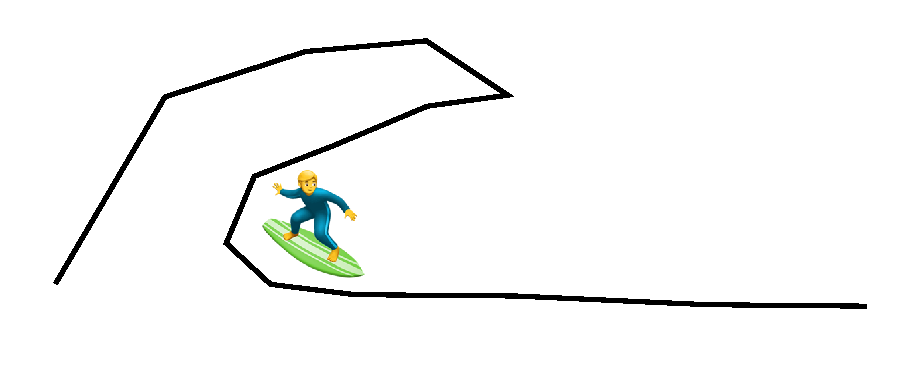
\includegraphics{figures/chap3/surf.pdf}
  \caption[Shreddie Getting Barreled]{Shreddie McShredface showing everyone how to get barreled.}
  \label{fig:TPM}
\end{figure*}

\lipsum[2]

\begin{table}[hbt!]\centering
\captionsetup{justification=centering}
\captionsetup{width=.6\textwidth}
\captionsetup{skip=2pt}
\caption{Wave Statistics}
\renewcommand{\arraystretch}{1.5}
\begin{threeparttable}
\begin{tabular}{cccc}\toprule
  {Wave Height} & {Awesomeness\tnote{a}} \\ \midrule
    1-2 & 4\\
    2-4 & 8\\
    4-6 & 10\\
    6-8 & 8\\
    8-10 & 6\tnote{b}\\ \bottomrule
\end{tabular}
\begin{tablenotes}
\item[a] \footnotesize Awesomeness is on a 1-10 scale, 1 being the min and 10 being the max awesomeness
\item[b] \footnotesize This would be higher if you weren't afraid for your life
\end{tablenotes}
\end{threeparttable}
\end{table}

\chapter{Outlook}

\section{Lessons Learned}

\begin{itemize}
  \item Do not eat directly before surfing
  \item Surf with a buddy
  \item Do not wax the bottom of the board

\end{itemize}

%\include{chap1}
%\include{chap2}

\appendix
\chapter{Appendix for Wave Physics}

\begin{equation}
\frac{1}{c^2}\frac{\partial^2\psi}{\partial t^2}=\frac{\partial^2\psi}{\partial x^2}
\label{eq:wave}
\end{equation}

% \chapter{More Monticello Candidates}
\printbibliography

\end{document}
